\documentclass{beamer}
\usetheme{Madrid}

\usepackage{amsmath, amssymb, amsthm}
\usepackage{graphicx}
\usepackage{listings}
\usepackage{gensymb}
\usepackage[utf8]{inputenc}
\usepackage{hyperref}
\usepackage{gvv}

\begin{document}

\title{matgeo: 1.4-9c}
\author{EE24BTECH11009 - Mokshith Kumar}
}
\frame{\titlepage}
\begin{frame}
\frametitle{Question}
 In what ratio does the point \brak{-4,6} divide the line segment joining the points $\vec{A}$\brak{-6,0} and $\vec{B}$\brak{3,-8}?\hfill{1.4-9c}
 \end{frame}
\begin{frame}
\frametitle{Plot}
\begin{figure}[h!]
   \centering
   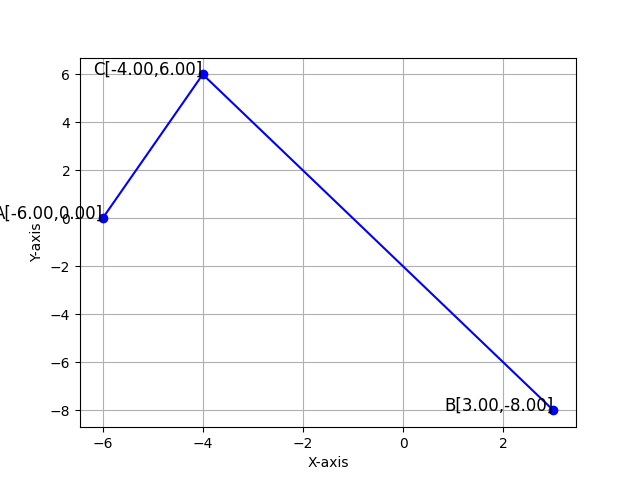
\includegraphics[width=0.7\linewidth]{figs/plot.png}
   \caption{ }
   \label{stemplot}
\end{figure}\\
\end{frame}
\begin{frame}
\frametitle{Solution}
\figref{stemplot} we can see that the given point doesn't lie on the line segment joining A and B.\\
\begin{align}
d_1&=\left\|{(A-C)}\right\|\\
\implies d_1^2&= (A-C)(A-C)^T\\
&=\myvec{
-2 & -6
}
\myvec{
-2\\
-6
}\\
\implies d_1&=\sqrt{40}\\
\end{align}
\begin{align}
d_2&=\left\|{(B-C)}\right\|\\
\implies d_2^2&=(B-C)(B-C)^T\\
&=\myvec{
7 & -14
}
\myvec{
7\\
-14
}\\
\implies d_2&=7\sqrt{5}\\
\therefore \frac{d_1}{d_2} &= \frac{\sqrt{40}}{7\sqrt{5}}
\end{align}
\end{frame}
\begin{frame}
\frametitle{Table}
\begin{table}[h]
    \centering
    \begin{tabular}{|c|c|}
        \hline
        Point & Coordinates\\
        \hline
        $A$ & \myvec{0\\6}\\
        \hline
        $B$ & \myvec{8\\0}\\
        \hline
        $C$ & \myvec{0\\0}\\
        \hline
\end{tabular}

    \caption{Parameter Table}
    \label{tab.1}
\end{table}
\end{frame}
\end{document}